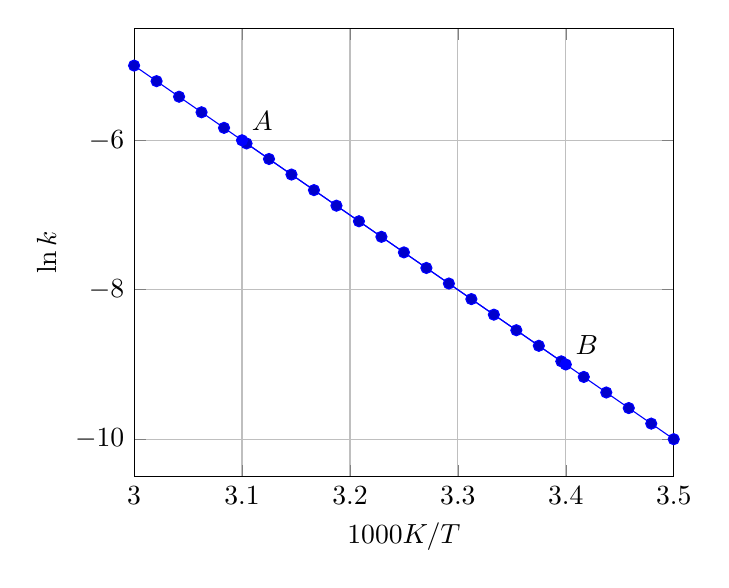
\begin{tikzpicture}
    \begin{axis}
        [
            grid = major,
            xlabel = {$\qty{1000}{K}/T$},
            ylabel = {$\ln k$},
            xmin = 3, xmax = 3.5,
            domain = 3:3.5,
        ]
    \addplot
        { -10*x + 25 };
    \addplot [mark=*, color=blue] coordinates
        { 
            (3.1,-6)
            (3.4,-9) 
        };
    \node [anchor = south west] at (axis cs:3.1,-6) 
        {$A$};
    \node [anchor = south west] at (axis cs:3.4,-9) 
        {$B$};
    \end{axis}
\end{tikzpicture}